\section{Elliptic Curves as Complex Tori}
\label{sec:over-C}

The goal of this section is to show an elliptic curve defined over $\C$
is isomorphic to a torus as a Riemann surface (and actually even 
as a complex lie group). In particular,
this will allow us to
verify that the point (d) of the Weil Conjectures is true for elliptic curves.

Throughout this section, we suppose $K = \C$.

\subsection{Riemann Surface Structure}

First, let's discuss the Riemann surface structure that an elliptic curve 
is given.

\begin{definition}
	The \emph{complex topology} on $\proj^n$ is the quotient topology induced
	by the Euclidean topology on $\C^{n+1}$.
\end{definition}

Throughout this section we will consider $\proj^n$ with the complex topology,
and hence an elliptic curve $E \subset \proj^2$ will be equipped with
the subspace topology.

\begin{proposition}
	\label{prop:riemann-surf-struct}
	Let $E \subset \proj^2$ be an elliptic curve, then $E$ admits
	the structure of a Riemann surface.
\end{proposition}

\begin{proof}
	Let $y^2 - x^3 - ax - b = f(x, y) = 0$ be the equation defining $E$.
	So for all $P = (x_P, y_P) \in E$ with $y_P \neq 0$,
	$\frac{\partial f}{\partial y}(P) \neq 0$ and hence by the implicit function
	theorem there exists an open set $V_P \subseteq \C$ containing $x_P$ and an
	analytic function $g_P: V_P \to \C$, such that $g_P(x_P) = y_P$ and
	$f(x, g_P(x)) = 0$ for all $x \in V_P$. 
	Furthermore $U_P = (\id\times g_P)(V_P) \subset E$,
	is an open subset of $E$. Indeed, $U_P = \pi_x^{-1}(V_P)$, where
	$\pi_x: E\setminus\{O\} \to \C, (x, y) \mapsto x$.
	Hence we define
	$\phi_P = \pi_x\vert_{U_P}$ which is a homeomorphism to its
	image $\phi_P(U_P) = V_P$ (the inverse to which is given by
	$x \mapsto (x, g_P(x))$).

	For all $P = (x_P, 0) \in E$ we define the chart $\phi_P: U_P \to \C$
	similarly, except we inverse the roles of $x$ and $y$ in the above reasoning.
	Indeed, $\frac{\partial f}{\partial x}(P) \neq 0$, since $E$ is smooth,
	hence we get the existence of $V_P \subset \C$ containing $y_P$ and
	$h_P: V_P \mapsto \C$, such that $h_P(y_P) = x_P$ and
	$f(h_P(y), y) = 0$ for all $y \in V_P$. We set
	$U_P := (h_P \times \id)(V_P)$ and 
	$\phi_P: U_P \to \C, (x, y) \mapsto y$.

	Finally, we have yet to define a chart whose domain covers the point at
	infinity $O = [0, 1, 0] \in E$. To do this, we can look at $E$
	in $\{[X, Y, Z] \in \proj^2 \mid Y \neq 0\}$ instead.
	We get that in this copy of $\A^2$, $E$ is given by
	the equation. 
	\begin{equation*}
		z - x^3 - axz^2 - bz^3 = \tilde f(x, z) = 0.
	\end{equation*}
	We have that $\frac{\partial \tilde f}{\partial z} (O) = 1 \neq 0$, hence we
	can again apply the reasoning from above. We obtain the chart
	$\phi_O: U_O \to \C, [x, 1, z] \mapsto x$ with inverse
	$\phi_0^{-1}: \phi_O(U_O) \to \C, x \mapsto [x, 1, \tilde g(x)]$.

	Now let $P, Q \in E \setminus \{O\}$, with $y_P \neq 0$ and $y_Q = 0$.
	We have that
	\begin{align*}
		\phi_P \circ \phi_Q^{-1} (y) &= \phi_P(h_Q(y), y) = h_Q(y)\\
		\phi_Q \circ \phi_P^{-1} (x) &= \phi_{Q}(x, g_P(x)) = g_P(x)\\
		\phi_P\circ \phi_O^{-1}(x) &= \phi_P([x, 1, \tilde g(x)])
		= \phi_P\left(\frac{x}{\tilde g(x)},
		\frac{1}{\tilde g(x)}\right) = \frac{x}{\tilde g(x)}\\
		\phi_O\circ \phi_P^{-1}(x) &= \phi_O(x, g_P(x))
		= \phi_O\left(\left[\frac{x}{g_P(x)}, 1, \frac{1}{g_P(x)}\right]\right)
		= \frac{x}{g_P(x)}
	\end{align*}
	All of these transition maps are holomorphic and by transitivity so are
	$\phi_O \circ \phi_Q^{-1}$ and $\phi_Q \circ \phi_O^{-1}$.
	Hence the the atlas $\mathcal{A} = \{\phi_P \mid P \in E\}$ is
	holomorphic
	and so gives $E$ the structure of a Riemann surface.
\end{proof}

\subsection{Elliptic Functions}

Let's introduce the definition and some basic properties of elliptic functions.
For the rest of this section,
let $\Lambda \subseteq \C$ be an arbitrary lattice.

\begin{definition}
	An \emph{elliptic function} (relative to the lattice $\Lambda$)
	is a meromorphic function
	$f$ on $\C$, which satisfies
	\begin{equation*}
		f(z + \lambda) = f(z)\qquad\textrm{ for all } \lambda \in \Lambda, z \in \C
	\end{equation*}
\end{definition}

\begin{notation}
	The set of elliptic functions relative to the lattice $\Lambda$ is denoted
	$\C(\Lambda)$.
\end{notation}

\begin{remark}
	$\C(\Lambda)$ is a field with the usual operations of 
	addition and multiplication of complex functions.
\end{remark}

\begin{definition}
	A \emph{fundamental parallelogram} for $\Lambda$ is a set of the form
	\begin{equation*}
		D = \{a + r \lambda_1 + s \lambda_2 \mid r, s \in [0, 1)\},
	\end{equation*}
	where $a \in \C$ and $\lambda_1, \lambda_2$ is a basis for $\Lambda$.
\end{definition}

Liouville's theorem tells us that a bounded entire function is constant.
If an elliptic function is bounded on a fundamental parallelogram, then
it is bounded everywhere by periodicity, so we get the following proposition.

\begin{proposition}
	\label{prop:no-poles}
	An elliptic function with no poles (or no zeros) is constant.
\end{proposition}

\begin{proof}
	Suppose that $f(z)\in \C(\Lambda)$ is holomorphic (i.e. it has no poles).
	Let $D$ be a fundamental
	parallelogram for $\Lambda$. Since $f$ is periodic, we have that
	\begin{equation*}
		\sup_{z \in \C}|f(z)| = \sup_{z \in \cl{D}}|f(z)|.
	\end{equation*}
	Since $f$ is continous, it is bounded on the compact set $\cl{D}$.
	It follows that it is bounded on all of $\C$.
	By Liouville's theorem, $f$ is constant.
	If $f$ has no zeros, we can look at $1/f$.
\end{proof}

\begin{notation}
	For $f \in \C(\Lambda), z \in \C/\Lambda$, we write $f(z), \res_z(f)$ and $\ord_z(f)$ for
	$f(\bar{z}), \res_{\bar{z}}(f)$ and $\ord_{\bar{z}}(f)$ respectively,
	for any one representative
	$\bar{z} \in \C$ of the coset $z$. This is well defined by the
	$\Lambda$-periodicity of $f$.
\end{notation}

From periodicity of an elliptic function, we can deduce the following result
from the residue theorem.

\begin{proposition}
	\label{prop:residue}
	Let $f \in \C(\Lambda)$.
	\begin{enumerate}[label=(\alph*)]
		\item $\sum_{z \in \C/\Lambda} \res_z(f) = 0$.
		\item $\sum_{z \in \C/\Lambda} \ord_z(f) = 0$.
	\end{enumerate}
\end{proposition}

\begin{proof}
	We can choose a fundamental parallelogram $D$ for $\Lambda$,
	such that $f$ has no zeroes or poles on the boundary $\partial D$.
	\begin{enumerate}[label=(\alph*)]
		\item By the residue theorem,
			\begin{equation*}
				\sum_{z \in \C\Lambda} \res_z(f)
				= \frac{1}{2\pi i}\int_{\partial D}f(z)\,dz.
			\end{equation*}
			By periodicity, the integrals along the opposite sides of $\partial D$
			cancel out, so the integral along the boundary of $D$ is zero.
		\item Since $f$ is periodic, so is $f'$ and hence also
			$f/f'$. We have that $\res_z(f/f') = \ord_z(f)$ and hence 
			this point follows from (a) applied to the elliptic function
			$f/f'$.
	\end{enumerate}
\end{proof}

Next let us introduce the Weierstrass $\wp$-function, which will serve
as a connecting link between elliptic curves and elliptic functions.

\begin{definition}
	\begin{enumerate}[label=(\alph*)]
		\item
			The Weierstrass
			elliptic function ($\wp$-function),
			is defined by the series
			\begin{equation*}
				\wp(z; \Lambda) = \frac{1}{z^2}
				+ \sum_{\lambda \in \Lambda\setminus\{0\}}
				\left(
					\frac{1}{(z-\lambda)^2} - \frac{1}{\lambda^2}
				\right)
			\end{equation*}
		\item
			The Eisenstein series (of $\Lambda$) of weight $k$,
			where $k \geq 2$ is an integer
			is the series
			\begin{equation*}
				G_k(\Lambda) = \sum_{\lambda \in \Lambda\setminus\{0\}}
				\lambda^{-k}
			\end{equation*}
	\end{enumerate}
\end{definition}

\begin{notation}
	If $\Lambda$ is known from context, we write simply
	$\wp(z)$ and $G_k$ for $\wp(z; \Lambda), G_k(\Lambda)$
	respectively.
\end{notation}

Of course, we have to show that the Eisenstein series converge
and the Weierstrass
$\wp$-function are well defined and elliptic.

% Theorem VI.3.1
\begin{proposition}
	\label{prop:wp-properties}
	\begin{enumerate}[label=(\alph*)]
		\item	The Eisenstein series $G_k(\Lambda)$ is absolutely convergent
			for all $k \geq 3$.
		\item The series defining the Weierstrass $\wp$-function converges
			absolutely and uniformly on every compact subset of
			$\C\setminus\Lambda$. It defines a meromorphic function on $\C$ with 
			double poles of residue 0 at each lattice point.
		\item The Weierstrass $\wp$-function is an even elliptic function.
	\end{enumerate}
\end{proposition}

\begin{proof}
	\begin{enumerate}[label=(\alph*)]
	\item	Let $\lambda_1, \lambda_2$ be basis vectors of $\Lambda$.
		Let 
		\begin{equation*}
			A_N := \{n\lambda_1 + m\lambda_2 \in \Lambda \mid
			n, m \in \Z, \max(|n|, |m|) = N\}.
		\end{equation*}
		Let also 
		\begin{equation*}
			m = \min\{|a\lambda_1 + b\lambda_2| \mid 
			a, b \in \R, \max(|a|,|b|) = 1\},
		\end{equation*}
		then $m$ is well defined and strictly positive,
		as it's the minimum of a compact subset of $\R$, which does
		not contain zero. We have that
		\begin{equation*}
			\#A_N = (2N + 1)^2 - (2N - 1)^2 = 8N.
		\end{equation*}
		Furthermore, $\min\{|\lambda|, \lambda \in A_N\} \geq Nm$, so we
		get
		\begin{equation*}
			\sum_{\lambda \in \Lambda\setminus 0}\frac{1}{|\lambda|^k}
			\leq \sum_{N=1}^\infty \frac{\#A_N}{\min\{|\lambda|, \lambda \in
			A_N\}^k}
			= \sum_{N=1}^{\infty} \frac{8}{m^kN^{k-1}} < \infty.
		\end{equation*}
	\item
		If $|\lambda| > 2|z|$, then we have that
		\begin{equation*}
			|2\lambda - z| \leq 2|\lambda| + |z| \leq \frac{5}{2}|\lambda|
		\end{equation*}
		and
		\begin{equation*}
			|z - \lambda| = |\lambda|\left|\frac{z}{\lambda} - 1\right| \geq
			\frac{1}{2}|\lambda|.
		\end{equation*}
		These imply that
		\begin{equation*}
			\left| \frac{1}{(z - \lambda)^2} - \frac{1}{\lambda^2}\right|
			= \left| \frac{z(2\lambda - z)}{\lambda^2(z - \lambda)^2}\right|
			\leq 10\frac{|z|}{|\lambda|^3}
		\end{equation*}
		Hence using (a) we see that
		the series for $\wp$ converges absolutely and uniformly on any 
		compact subset of $\C \setminus \Lambda$. It follows that
		the series defines a holomorphic function on $\C \setminus \Lambda$,
		furthermore, it is clear from the series expansion that $\wp$ has
		a double pole with residue $0$ at each point of $\Lambda$.
	\item It follows from the definition of $\wp$ that
		$\wp(z) = \wp(-z)$, since we can just replace $\lambda$ by 
		$-\lambda$ in the sum. Since the series converges uniformly,
		we can compute the derivative of $\wp$ by termwise differentiation.
		We obtain
		\begin{equation*}
			\wp'(z) = -2\sum_{\lambda \in \Lambda} \frac{1}{(z - \lambda)^3}.
		\end{equation*}
		It is clear from this expansion that $\wp'$ is an elliptic function,
		hence for all $\lambda \in \Lambda$,
		\begin{equation*}
			\frac{\partial}{\partial z}(\wp(z) - \wp(z + \lambda))
			= \wp'(z) - \wp'(z + \lambda) = 0
		\end{equation*}
		and hence $\wp(z) - \wp(z + \lambda)$ is the constant function.
		By setting $z = -\lambda/2$, and using the fact $\wp$ is even,
		we get that
		\begin{equation*}
			\wp(z) - \wp(z + \lambda) = \wp(-\lambda/2) - \wp(\lambda/2) = 0
		\end{equation*}
		and hence $\wp$ is an elliptic function.
	\end{enumerate}
\end{proof}

As in the case of curves, we can define divisors for elliptic
functions.
\begin{definition}
	Let $\Lambda$ be a lattice, the \emph{divisor group}
	$\Div(\C/\Lambda)$ to be the free abelian group on the set
	$\C/\Lambda$. We write elements of $\Div(\C/\Lambda)$ as
	$\sum_{z \in\C/\Lambda} n_z(z)$ with $n_z \in \Z$ and
	$n_z = 0$ for all but finitely many $z$.

	We define analogously to the case of elliptic curves,
	\begin{align*}
		\deg D &= \sum_{z \in \C/\Lambda} n_z\\
		\Div^0(\C/\Lambda) &= \{D \in \Div(\C/\Lambda): \deg D = 0\}
	\end{align*}
	and for any $f \in \C(\Lambda)^\times$ we define the divisor
	$\div(f) \in \Div^0(\C/\Lambda)$ by
	\begin{equation*}
		\div(f) = \sum_{z \in \C/\Lambda} \ord_z(f)\cdot(z)
	\end{equation*}
\end{definition}

Divisors give us an useful way to compare elliptic functions, as if
the divisors of two elliptic functions are equal, the functions have
to be equal up to multiplication by a constant.
In fact, we can use them to show the following powerful result.

\begin{theorem}
	\label{thm:wp-generates}
	We have that
	\begin{equation*}
		\C(\Lambda) = \C(\wp, \wp')
	\end{equation*}
\end{theorem}

\begin{proof}
	Let $f \in C(\Lambda)$. We can decompose $f$ as
	\begin{equation*}
		f(z) = \frac{1}{2}(f(z) + f (-z)) + \frac{1}{2}(f(z) - f(-z)),
	\end{equation*}
	hence we see that it suffices to prove the theorem for odd and even
	functions. If $f$ is odd, then $\wp'f$ is even, so we can just consider
	the case that $f$ is even.

	If $f$ is even, we have that
	\begin{equation*}
		\ord_z f = \ord_{-z} f
	\end{equation*}
	for all $z\in \C$. Furthermore, if $2z \in \Lambda$, then
	$\ord_z f$ is even. By differentiating $f(z) = f(-z)$ repeatedly,
	we obtain
	\begin{equation*}
		f^{(k)}(z) = (-1)^kf^{(k)}(-z)
	\end{equation*}
	so if $2z \in \Lambda$, $f^{(k)}(z) = f^{(k)}(-z)$, which implies
	$f^{(k)}(z) = 0$ for all odd $k$. Hence $\ord_z f$ must be even.

	Let $D$ be a fundamental parallelogram for $\Lambda$ and let $H$ 
	be ``half" of $D$ in the sense that it is a fundamental domain for
	$(\C/\Lambda)/\{\pm 1\}$ in $\C$,
	i.e. $\C = (H + \Lambda) \cup (-H + \Lambda)$.
	Then the divisor of $f$ has the form
	\begin{equation*}
		\sum_{z \in D} n_z(z) = \sum_{z \in H} n'_z((z) + (-z)).
	\end{equation*}
	for certain integers $n_z$ and
	\begin{equation*}
		n'_z =
		\begin{cases}
			n_z &\textrm{if } 2z \notin \Lambda;\\
			\frac{1}{2}n_z &\textrm{if } 2z \in \Lambda.
		\end{cases}
	\end{equation*}
	If $2z \in \Lambda$, then
	$n_z = \ord_z f$ is even, so this is well defined.

	Now consider the function
	\begin{equation*}
		g(z) = \prod_{w \in H\setminus 0}(\wp(z) - \wp(w))^{n_w}.
	\end{equation*}
	The divisor of $\wp(z) - \wp(w)$ is $(w) + (-w) - 2(0)$, so we see that
	$f$ and $g$ have exactly the same zeros and poles except possibly at
	$0$. But then by \ref{prop:residue} they also have the same order at $0$.
	It follows that $f/g$ is a holomorphic elliptic function and so is constant
	by \ref{prop:no-poles}.
	We conclude that $f = cg \in \C(\wp, \wp')$.
\end{proof}

We would like to get a result similar to \ref{prop:div-principal} for
divisors of elliptic functions. In fact, such a result holds, and to show
it, we will make use of the Weierstrass $\sigma$-function.

\begin{definition}
	The \emph{Weierstrass $\sigma$-function} (relative to $\Lambda$) is the
	function defined by
	\begin{equation*}
		\sigma(z; \Lambda) = z \prod_{\lambda\in\Lambda\setminus 0}
		\left(1 - \frac{z}{\lambda}\right)
		\exp\left(\frac{z}{\lambda} + \frac{1}{2}\left(\frac{z}{\lambda}\right)^2\right)
	\end{equation*}
\end{definition}

\begin{notation}
	As before, we write just $\sigma(z)$ for $\sigma(z; \Lambda)$ when $\Lambda$
	is clear from context.
\end{notation}

% Characterization of principal divisors.

The most useful property of the $\sigma$-function is that it holomorphic
and has simple zeroes on the lattice points. This will allow us to take
an appropriate product of $\sigma$ translated to match the zeroes and poles
of any given elliptic function. Furthermore, if certain criteria are met,
this product will define an elliptic function.

\begin{lemma}
	\label{lem:sigma-properties}
	\begin{enumerate}[label=(\alph*)]
		\item The infinite product for $\sigma$ defines a holomorphic function
			on all of $\C$. It has simple zeros at each $z \in \Lambda$
			and no other zeros.
		\item For all $z \in \C\setminus \Lambda$
			\begin{equation*}
				\frac{d^2}{dz^2}\log\sigma(z) = -\wp(z)
			\end{equation*}
		\item For any $\lambda \in \Lambda$, there are constants
			$a, b \in \C$ such that for all $z\in \C$
			\begin{equation*}
				\sigma(z + \lambda) = e^{az + b}\sigma(z)
			\end{equation*}
	\end{enumerate}
\end{lemma}

\begin{proof}	
	\begin{enumerate}[label=(\alph*)]
		\item Let $K \subset \C$ be a compact set.
			Let $M > 0$ be such that $K \subset B(0, M)$.
			We have that for all $z \in K$ and
			$\lambda \in \Lambda\setminus 0$ such that
			$|\lambda| \geq \frac{3}{2}M$,
			using the Taylor expansion of $\log(1 - x)$,
			\begin{align*}
				\left|\log\left(1 - \frac{z}{\lambda}\right) +
				\frac{z}{\lambda} + \frac{1}{2}\left(
				\frac{z}{\lambda}\right)^2\right|
				&\leq \sum_{k = 3}^\infty
				\frac{1}{k}\left|\frac{z}{\lambda}\right|^k\\
				\left(\textrm{since $\left|\frac{z}{\lambda}\right|
					\leq \frac{M}{|\lambda|}$}
				\right)\qquad
				&\leq \frac{1}{3}\left(\frac{M}{|\lambda|}\right)^3
				\sum_{k = 0}^\infty\left(\frac{M}{|\lambda|}\right)^k\\
				&= \frac{1}{3}\left(\frac{M}{|\lambda|}\right)^3
				\left(1 - \frac{M}{|\lambda|}\right)^{-1}\\
				\left(\textrm{since $\frac{M}{|\lambda|} \leq \frac{2}{3}$}
				\right)\qquad
				&\leq \left(\frac{M}{|\lambda|}\right)^3
			\end{align*}
			We deduce from \ref{prop:wp-properties}(a) that the series
			\begin{equation*}
				\sum_{\substack{
					\lambda \in \Lambda\setminus 0\\
					|\lambda| \geq \frac{3}{2}M}}
				\left|\log\left(1 - \frac{z}{\lambda}\right) +
				\frac{z}{\lambda} + \frac{1}{2}\left(
				\frac{z}{\lambda}\right)^2\right|
			\end{equation*}
			converges uniformly on $K$
			and hence so does the product defining $\sigma$ 
			(since there is only a finite number of $\lambda \in \Lambda$ with
			$|\lambda| < \frac{3}{2}M$).

			Hence the product defining $\sigma$ converges on all compact subsets
			of $\C$ and so $\sigma$ defines a holomorphic function
			on all of $\C$.
			
			Since the series
			\begin{equation*}
				\sum_{\lambda \in \Lambda\setminus 0}
				\left(\log\left(1 - \frac{z}{\lambda}\right) +
				\frac{z}{\lambda} + \frac{1}{2}\left(
			\frac{z}{\lambda}\right)^2\right)
			\end{equation*}
			converges provided $z \notin \Lambda$, $\sigma(z) \neq 0$ for all
			$z \in \Lambda$. Clearly, $\sigma(\lambda) = 0$ for all
			$\lambda \in \Lambda$ and $\frac{\sigma(z)}{z - \lambda}$ is non-zero
			for $z = \lambda$ by the same argument as above. Hence $\sigma$
			has simple zeros at each $z \in \Lambda$ and no other zeros.

		\item We have from (a) that we can differentiate
			\begin{equation*}
				\log \sigma(z) = \log z + 
				\sum_{\lambda \in \Lambda\setminus 0}
				\left(\log\left(1 - \frac{z}{\lambda}\right) +
				\frac{z}{\lambda} + \frac{1}{2}\left(
				\frac{z}{\lambda}\right)^2\right)
			\end{equation*}
			term by term.
			We get
			\begin{align*}
				\frac{d}{dz} \log \sigma(z)
				&= \frac{1}{z} +
				\sum_{\lambda \in \Lambda \setminus 0}
				\left(\frac{1}{z - \lambda}
				+ \frac{1}{\lambda} + \frac{z}{\lambda^2}\right)\\
				\frac{d^2}{dz^2} \log \sigma(z)
				&= -\frac{1}{z^2} + \sum_{\lambda \in \Lambda\setminus 0}
				\left(\frac{-1}{(z - \lambda)^2} + \frac{1}{\lambda^2}\right)
				= -\wp(z)
			\end{align*}

		\item Let $\lambda \in \Lambda$. Since $\wp$ is elliptic,
			for all $z \in \C$,
			\begin{equation*}
				\frac{d^2}{dz^2}\log\sigma(z + \lambda)
				= -\wp(z + \lambda) = \wp(z)
				= \frac{d^2}{dz^2}\log\sigma(z).
			\end{equation*}
			By integrating twice, we obtain
			\begin{equation*}
				\log \sigma(z + \lambda) = \log\sigma(z) + az + b
			\end{equation*}
			for some constants of integration $a, b \in \C$.
	\end{enumerate}
\end{proof}

We will now see how we can use the $\sigma$-function to prove the desired
property.

\begin{proposition}
	\label{prop:complex-divisors}
	Let $n_1, \dots, n_r \in \Z$ and $z_1, \dots, z_n \in \C$, such that
	\begin{equation*}
		\sum n_i = 0 \textrm{ and } \sum n_iz_i \in \Lambda.
	\end{equation*}
	Then there exists an elliptic function $f(z) \in \C(\Lambda)$ satisfying
	\begin{equation*}
		\div(f) = \sum n_i(z_i).
	\end{equation*}
\end{proposition}

\begin{proof}
	Let $\lambda = \sum n_i z_i \in \Lambda$.
	Replacing $\sum n_i(z_i)$ by $\sum n_i(z_i) + (0) - (\lambda)$,
	we may assume
	that $\sum n_iz_i = 0$ (indeed these are two different writings
	for the same divisor as $0 \equiv \lambda \mod \Lambda$).
	Then from \ref{lem:sigma-properties}(a) we get that
	\begin{equation*}
		f(z) = \prod \sigma(z - z_i)^{n_i}
	\end{equation*}
	has the correct zeros and poles.
	Furthermore, from \ref{lem:sigma-properties}(c),
	we get that
	\begin{align*}
		f(z + \lambda) &= \prod \sigma(z + \lambda - z_i)^{n_i}\\
		&= \prod \left(\sigma(z - z_i)e^{a(z - z_i) + b}\right)^{n_i}\\
		&= e^{\sum n_i(az + b) - a\sum n_iz_i} f(z)\\
		&= f(z)
	\end{align*}
	and hence $f \in \C(\Lambda)$.
\end{proof}

\subsection{Constructing the Isomorphism}

The Weierstrass $\wp$-function satisfies a differential equation, which we
will be able exploit to exhibit an isomorphism between an elliptic curve
and a torus.

\begin{proposition}
	\label{prop:diffeq}
	For all $z \in \C \setminus \Lambda$, we have that
	\begin{equation*}
		\wp'(z)^2 = 4\wp(z)^3 - 60G_4\wp(z) - 140G_6
	\end{equation*}
\end{proposition}

In order to show that $\wp$ satisfies this differential equation,
we will first calculate the Laurent series of $\wp$.

\begin{proposition}
	\label{prop:laurent}
	The Laurent series for $\wp(z)$ about $z = 0$ is given by
	\begin{equation*}
		\wp(z) = z^{-2} + \sum_{k = 1}^\infty (2k + 1)G_{2k + 2}z^{2k}.
	\end{equation*}
\end{proposition}
\begin{proof}
	For $|z| < |\lambda|$, we have that
	\begin{align*}
		\frac{1}{(z - \lambda)^2} - \frac{1}{\lambda^{2}}
		&= \frac{1}{\lambda^2}\left(\left(\frac{1}{1 - \frac{z}{\lambda}}
			\right)^2 - 1\right)\\
		&= \frac{1}{\lambda^2}\left(\left(
		\sum_{k = 0}^{\infty}\left(\frac{z}{\lambda}\right)^k\right)^2 -
		1 \right)\\	
		&= \frac{1}{\lambda^2}\left(
		\sum_{k = 0}^\infty(k + 1)\left(\frac{z}{\lambda}\right)^k - 1\right)\\
		&= \sum_{k = 1}^\infty (k + 1)\frac{z^k}{\lambda^{k+ 2}}
	\end{align*}
	where the third equality is obtained by grouping the terms
	$\left(\frac{z}{\lambda}\right)^k$ together in the double sum 
	(the series is absolutely convergent). Hence we have that
	for all $|z| < \min\{|\lambda|: \lambda \in \Lambda\setminus 0\}$
	\begin{align*}
		\wp(z) &= z^{-2} + \sum_{\lambda\in \Lambda \setminus 0}
		\left((z - \lambda)^{-2} - \lambda^{-2}\right)\\
		&= z^{-2} + \sum_{\lambda\in \Lambda\setminus 0}
		\sum_{k = 1}^\infty(k + 1)\frac{z^k}{\lambda^{k + 2}}\\
		&= z^{-2} + \sum_{k = 1}^{\infty}(k + 1)z^k G_{k + 2}
	\end{align*}
	The result follows from the fact that $G_{k + 2} = 0$ for $k$ odd, since
	the terms $1/\lambda^{k + 2}$ and $1/(-\lambda)^{k + 2}$ cancel each other
	out.
\end{proof}

We can now use the Laurent series to show that $\wp$ satisfies
\ref{prop:diffeq}.
Since an elliptic function with no poles is constant, it suffices to look
at the first few terms of the Laurent series.

\begin{proof}[Proof of \ref{prop:diffeq}]
	We write the first few terms in various Laurent expansions:
	\begin{align*}
		\wp(z) &= z^{-2} + 3G_4z^2 + 5G_6z^4 + \dots\\
		\wp(z)^3 &= z^{-6} + 9G_4z^{-4} + 15G_6 + \dots\\
		\wp'(z)^2 &= 4z^{-6} - 24G_4z^{-2} - 80G_6 + \dots
	\end{align*}
	Comparing these, we see that the function
	\begin{equation*}
		f(z) = \wp'(z)^2 - 4\wp(z)^3 + 60G_4\wp(z) + 140G_6
	\end{equation*}
	is holomorphic around $z = 0$, since the negative power terms cancel
	each other out. But since $\wp$ is elliptic and holomorphic on $\C \setminus
	\Lambda$, we get that $f$ is elliptic and holomorphic everywhere,
	so constant.
	Since $f$ vanishes at $0$, we get $f\equiv 0$.
\end{proof}

\begin{remark}
	We write
	\begin{equation*}
		g_2 = g_2(\Lambda) = 60G_4
		\textrm{ and }
		g_3 = g_3(\Lambda) = 60G_3.
	\end{equation*}
	Then the equation in \ref{prop:diffeq} becomes
	\begin{equation*}
		\wp'(z)^2 = 4\wp(z)^3 - g_2\wp(z) - g_3
	\end{equation*}
\end{remark}

The differential equation in \ref{prop:diffeq} being the equation for
an elliptic curve, we can finally exhibit an isomorphism between
$\C/\Lambda$, which is the torus and the elliptic curve given by the
corresponding equation.

% Proposition VI.3.6
\begin{theorem}
	\label{thm:lattice-curve}
	Let $g_2, g_3$ be the quantities associated to $\Lambda$ as in the above
	remark.
	Let $E/\C$ be the curve given by the equation
	\begin{equation*}
		E: y^2 = 4x^3 - g_2 x - g_3
	\end{equation*}
	then $E$ is an elliptic curve and the map
	\begin{align*}
		\phi: \C/\Lambda &\to E\\
		z &\mapsto 
		\begin{cases}
			[\wp(z), \wp'(z), 1] &\textrm{if } z \not\in \Lambda\\
			[0, 1, 0] &\textrm{if } z \in \Lambda
		\end{cases}
	\end{align*}
	is an isomorphism of complex Lie groups.
\end{theorem}

\begin{proof}
	To show $E$ is an elliptic curve, we have to show that it is non-singular.	
	From \ref{prop:singular-determinant} this is the case if and only if
	the determinant $\Delta$ of the polynomial $f(x) = 4x^3 - g_2x - g_3$
	is non-zero, in other words if and only if $f$ has no repeated roots. 
	Let $\{\lambda_1, \lambda_2\}$ be a basis of $\Lambda$,
	let $\lambda_3 = \lambda_1 + \lambda_2$. then since $\wp'$ is
	an odd elliptic function, we have that for $i \in \{1, 2, 3\}$
	\begin{equation*}
		\wp'(\lambda_i/2) = -\wp'(-\lambda_i/2) = -\wp'(\lambda_i/2)
	\end{equation*}
	and hence $\wp'(\lambda_i/2) = 0$. It follows from $\ref{prop:diffeq}$
	that $\wp(\lambda_i/2)$ is a root of $f$. So we need to show that the
	$\wp(\lambda_i/2)$ are all distinct.
	The function $\wp(z) - \wp(\lambda_i/2)$ has a double zero at $\lambda_i/2$,
	since its derivative is $\wp'(z)$ which vanishes at $\lambda_i/2$.
	Using \ref{prop:residue} and \ref{prop:wp-properties}, we deduce that these
	are the only zeroes and hence the $\wp(\lambda_i/2)$ are all distinct.
	Hence $E$ is indeed an elliptic curve.

	The image of $\phi$ is contained in $E(\C)$ by \ref{prop:diffeq}.
	Let $[x, y, 1] \in E(\C)$, then we have that $\wp(z) - x$ is a non-constant
	elliptic function, so by \ref{prop:no-poles}, it has a zero $a \in \C$.
	Hence $\wp(a) = x$ and hence by \ref{prop:diffeq}, 
	\begin{equation*}
		\wp'(a)^2 = f(\wp(a)) = f(x) = y^2.
	\end{equation*}
	It follows that $\wp'(a) = \pm y$, hence by replacing $a$ with $-a$ in
	the case $\wp'(a) =-y$, we get that $\wp'(a) = y$.
	Hence $\phi(a) = [x, y, 1]$. This shows the surjectivity of $\phi$.

	Now to show injectivity, suppose $z_1, z_2 \in \C$ are such that
	$\phi(z_1) = \phi(z_2)$. Suppose $z_1 \not\equiv -z_1 \mod \Lambda$.
	The function $\wp(z) - \wp(z_1)$ admits the roots $z_1, -z_1, z_2$, but being
	of order 2, two of these values are congruent mod $\Lambda$.
	Hence $z_2 \equiv \pm z_1 \mod \Lambda$. But since
	$\wp'(z_1) = \wp'(z_2)$, we get necessarily $z_2 \equiv z_1 \mod \Lambda$.
	
	Now, if $z_1 \equiv -z_1 \mod \Lambda$, then
	\begin{equation*}
		\frac{\partial}{\partial z}(\wp(z) - \wp(z_1)) = \wp'(z)
	\end{equation*}
	and $\wp'(z_1) = \wp'(-z_1) = -\wp'(z_1)$ and hence $\wp'(z_1) = 0$.
	It follows that $z_1$ is a double root of $\wp(z) - \wp(z_1)$, which is of
	order 2. Hence $z_2$, being also a root of $\wp(z) - \wp(z_1)$, is
	necessarily congruent to $z_1$ mod $\Lambda$. This shows the injectivity
	of $\phi$.

	Now we will show $\phi$ is an isomorphism of Riemann surfaces.
	Denote by $\xi: \C \mapsto \C/\Lambda$, the quotient map.
	Then the charts of $\C/\Lambda$ are given by local sections of $\xi$.
	Let $z \in \C$ and $U \subseteq \C$ containing $z$ an open set such that 
	$\xi\vert_U$ is injective. Let $\psi$ be a chart of $E$
	which we can suppose (up to shrinking $U$) to be defined on
	$\phi(\xi(U))$.
	Depending on the value of $P = \phi(\xi(z))$, $\psi$ will be of one of the
	three forms as described in the proof of 
	Proposition \ref{prop:riemann-surf-struct}.
	We get that
	\begin{equation*}
		\psi\circ\phi\circ\xi = 
		\begin{cases}
			\wp &\textrm{ if } P \neq O\textrm{ and }\wp'(z) \neq 0\\
			\wp' &\textrm{ if } P \neq O\textrm{ and }\wp'(z) = 0\\
			\frac{\wp}{\wp'} &\textrm{ if }P = O
		\end{cases}
	\end{equation*}
	and hence $\psi\circ\phi\circ\xi$ is holomorphic (and seen as a map to its
	image, it is bijective, and hence biholomorphic). Since $\phi$ is
	bijective and locally biholomorphic, it is
	biholomorphic and hence an isomorphism of Riemann surfaces.
	
	Finally, we want to show that $\phi$ is a group homomorphism.
	Let $z_1, z_2 \in \C$, then from \ref{prop:complex-divisors}, there exists
	a function $f \in \C(\Lambda)$ with divisor
	\begin{equation*}
		\div(f) = (z_1 + z_2) - (z_1) - (z_2) + (0)
	\end{equation*}
	Now, by \ref{thm:wp-generates}, we can write $f(z) = F(\wp(z), \wp'(z))$ for
	some rational function $F(X, Y) \in \C(X, Y)$. We can see $F$ in
	\begin{equation*}
		\C(E) = \C(E\cap \A^2) = \Frac\left(\C[x, y]/(y^2 - 4x^3 + g_2x + g_3)\right)	
	\end{equation*}
	and hence $f = F \circ \phi$. It follows that
	\begin{equation*}
		\div (F) = (\phi(z_1 + z_2)) - (\phi(z_1)) - (\phi(z_2)) + (0)
	\end{equation*}
	By Proposition \ref{prop:div-principal}, it follows that
	\begin{equation*}
		\phi(z_1 + z_2) = \phi(z_1) + \phi(z_2)
	\end{equation*}
\end{proof}

The following theorem (which we will not prove) gives the converse to \ref{thm:lattice-curve}

% Theorem VI.5.1
\begin{theorem}
	\label{thm:curve-lattice}
	Let $E/\C$ be a non-singular curve given by the equation
	\begin{equation*}
		E: y^2 = 4x^3 - ax - b.
	\end{equation*} 
	Then there exists a lattice
	$\Lambda \subseteq \C$ unique up to homothety, such that
	$a = g_2(\Lambda)$ and $b = g_3(\Lambda)$
\end{theorem}

\subsection{Homology Groups of Elliptic Curves}

Since any elliptic curve is isomorphic to a curve given by an equation as in
\ref{thm:curve-lattice}, we deduce that all curves are homeomorphic
to a torus $\T^2$. This allows us to calculate its homology groups.

To calculate the homology groups of a torus, we will use simplicial homology,
as in \cite[\S2.1]{hatcher}. The torus can be given a $\Delta$-complex structure
as in Figure \ref{fig:torus-delta}.
\begin{figure}[h]
	\centering 
	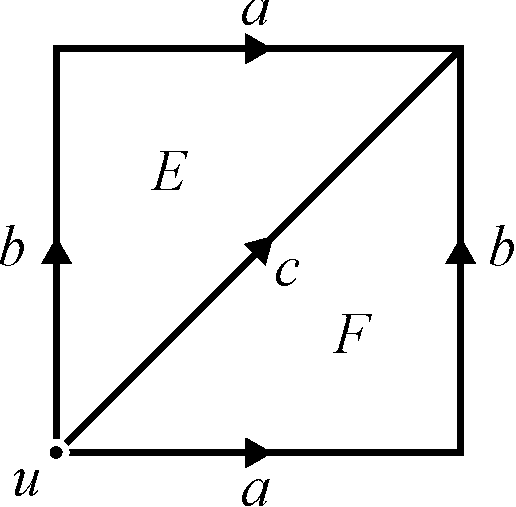
\includegraphics[width=0.4\columnwidth]{torus-delta.pdf}
	\caption[torus-delta]{$\Delta$-complex structure of a torus}
	\label{fig:torus-delta}
\end{figure}

The associated chain complex for taking simplicial homology is 
\begin{equation*}
	\begin{tikzcd}[row sep=tiny]
	\cdots & 0 & {E\Z \oplus F\Z} & {a\Z\oplus b\Z\oplus c\Z} & u\Z & 0 \\
	&&& {a,b,c} & 0 \\
	&& {E,F} & {a +b-c}
	\arrow["\partial_1", from=1-4, to=1-5]
	\arrow["\partial_2", from=1-3, to=1-4]
	\arrow[from=1-5, to=1-6]
	\arrow[from=1-2, to=1-3]
	\arrow[from=1-1, to=1-2]
	\arrow[maps to, from=3-3, to=3-4]
	\arrow[maps to, from=2-4, to=2-5]
\end{tikzcd}
\end{equation*}
Hence we get that
\begin{align*}
	H_0(\T^2) &\cong \Z,\\
	H_1(\T^2) &= \ker \partial_1 / \im \partial_2
	= a\Z \oplus b\Z \oplus c\Z / (a + b - c)\Z \cong \Z^2,\\
	H_2(\T^2) &= \ker \partial_2 = (E-F)\Z \cong \Z,
\end{align*}
and $H_n(\T^2) = 0$ for $n \geq 3$.
We deduce that the associated Betti numbers are
\begin{align*}
	b_0(\T^2) &= \rk(\Z) = 1,\\
	b_1(\T^2) &= \rk(\Z^2) = 2,\\
	b_2(\T^2) &= \rk(\Z) = 1,
\end{align*}
and $b_n(\T^2) = 0$ for $n \geq 3$.

Now if $E$ is given by a Weierstrass equation
defined over a number field embedded
in $\C$ and can be reduced modulo $p$ such that the curve
$C/\F_q$ obtained is a good reduction (i.e. an elliptic curve),
these Betti numbers coincide with
the degrees of the polynomials that appear in the decomposition of
$Z(C/\F_q)$, which was calculated in Theorem \ref{thm:weil-elliptic}.
This shows that part (e) of the Weil Conjectures
(\ref{thm:weil}) holds for the case of elliptic curves given by a Weierstrass
equation.
